%----------------------------------------------------------------------------------------
%	PACKAGES AND OTHER DOCUMENT CONFIGURATIONS
%----------------------------------------------------------------------------------------

\documentclass{article} % Paper and 12pt font size
\usepackage[utf8]{inputenc}
\usepackage{lmodern} % Use font Latin Modern Sans Typewriter
\usepackage[a4paper, margin=1in]{geometry} % Paper size and margin

\usepackage{enumitem} % Format the enumerated list
\usepackage{amsmath,amsfonts,amsthm,mathtools} % Math packages
\setlength\parindent{0pt} % Removes all indentation from paragraphs - comment this line for an assignment with lots of text

\usepackage{array}
\usepackage{tabu} % Table to text width
\renewcommand{\arraystretch}{0.6} % If the value is 1.0, the height of each row in the table is set to 1.5 relative to its default height. Adjust based on that.
\usepackage[table]{xcolor}

\usepackage{tikz} % Remember picture
\usepackage{graphicx} % Includes images
\graphicspath{ {./images/} } % Tells LATEX that the images are kept in a folder named images under the directory of the main document
\usepackage{subcaption}
\usepackage{wrapfig} % Wrap image i
\usepackage{eso-pic} % used for image background on titlepage

% Code listing style --------------
\usepackage{listings} % Code listing
\usepackage{color}
\definecolor{codegreen}{rgb}{0,0.6,0}
\definecolor{codegray}{rgb}{0.5,0.5,0.5}
\definecolor{codepurple}{rgb}{0.58,0,0.82}
\definecolor{backcolour}{rgb}{0.95,0.95,0.92}
\lstdefinestyle{mystyle}{
    backgroundcolor=\color{backcolour},
    commentstyle=\color{codegreen},
    basicstyle=\ttfamily\small,
    keywordstyle=\color{magenta},
    numberstyle=\tiny\color{codegray},
    stringstyle=\color{codepurple},
    breakatwhitespace=false,
    breaklines=true,
    captionpos=b,
    keepspaces=true,
    numbers=left,
    numbersep=5pt,
    showspaces=false,
    showstringspaces=false,
    showtabs=false,
    tabsize=2
}
\lstset{style=mystyle}

%----------------------------------------------------------------------------------------
%	TITLE SECTION
%----------------------------------------------------------------------------------------
\title{\Huge \textbf{Neural Network Classification \\ on the MNIST Dataset} \vspace{.4in} \hrule}

\author{%\LARGE University of Toronto Institute for Aerospace Studies\\
  \vspace{0.5cm}
	\Large ROB313: Introduction to Learning from Data \\
  \vspace{0.5cm}
	\Large Yizhi (Jojo) Zhou, 1003002396\\
}
\date{\normalsize\today}

\linespread{1.5}

\begin{document}
	\begin{titlepage}
	\tikz[remember picture,overlay]
	\node[yshift=8.0cm] at (current page.south){
\includegraphics[width=\paperwidth]{BG.png}};%height=\paperheight and (current page.south)
	\vspace*{3.5cm}
  {\let\newpage\relax\maketitle}
	\vspace*{\fill}

	\end{titlepage}

\newpage

%----------------------------------------------------------------------------------------
%	PROBLEM 1
%----------------------------------------------------------------------------------------
\vspace{0.3cm}
\section*{Objectives} % The * makes it an unnumbered section
In this project, a fully connected neural network with two hidden layers on the MNIST small dataset using a categorical (generalized Bernoulli) likelihood. The weights and bias parameters of the neural network are trained using stochastic gradient descent with a minibatch size of 250. The following report briefly describes the implementation of the neural network, studies the training process with different training sets and configurations, as long as the data points that are harder to predict with this model.


%----------------------------------------------------------------------------------------
%	PROBLEM 1
%----------------------------------------------------------------------------------------
\vspace{0.3cm}
\section*{Solution Structure and Strategies} % The * makes it an unnumbered section
The implemention is composed of the following 3 parts, with more details in the Jupyter Notebook\footnote{The Jupyter Notebook is attached in the submitted folder.}:
\begin{itemize}
  \item \textbf{Constructing the Neural Network}
    \begin{itemize}
    \item \textit{Forward Pass.} This function cumputes the forward pass of neural network consisting of two linear layers with log-softmax activation function. \textbf{To ensure numerical stability, the \textit{softmax} function shifts all the values by the magnitude of the largest value so that 0 becomes the largest number in each row and all the others are negative, and thus overflow due to the exponential is impossible.} Then, it simply uses broadcasting to divide each exponential by the sum of all 10 values in its row, and returns the class-conditional log probability for each of the 10 classes: $\hat f_j (x^{(i)}; w) = Pr(y^{(i)}_j=1\| x, w)$.

    \item \textit{Negative Log Likelihood.} This function takes in the outputs from \textit{Forward Pass} as $ \hat f$, and outouts the negative log likelihood of the categorical likelihood: $\frac{1}{N}\prod_{i=1}^N \prod_{j=1}^K \hat f_j (x^{(i)}; w)^{y^{(i)}}$
    \end{itemize}

  \item \textbf{Training the Parameters}
  \begin{itemize}
    \item \textit{Parameter Initialization.} The biases of the model are initialized to zero and the weights are initialized using Xavier initialization.

    \item \textit{Stochastic Gradient Descent.} This function starts with the initial parameters and then iterates through the minibatches of size 250 in a randomly shuffled training set, until it reaches the convergence, which is either the iteration cap of 10000 or the \textbf{early stopping criteria: the difference between two negative log likelihoods being smaller than an error bound twice, or the negative log likelihood being higher than the minimum for 5 times, or a combination of both.} The selection of this criteria is further discussed in the next section.
  \end{itemize}

  \item \textbf{Prediction and Visualization}
  \begin{itemize}
    \item \textit{Prediction.} The prediction is done simply by performing a forward pass with the trained parameters and the desired set (eg. validation or test set), which gives a the log likelihood of each class, for each datapoint. The class prediction for each datapoint is then the one with the highest log likelihood. If required, this function also shows the images from MNIST that are predicted wrong or have relatively low likelihoods.

    \item \textit{Image Visualization.} This function takes in the indices of desired datapoints, reshapes the features which represents the grey scale pixals, and turns them into images with labels. Note that these images are inverted in terms of black and white compared to those produced by the \textit{plot\_digit} function.
  \end{itemize}
\end{itemize}



%----------------------------------------------------------------------------------------
%	PROBLEM 1
%----------------------------------------------------------------------------------------
\vspace{0.3cm}
\section*{Performance and Discussion} % The * makes it an unnumbered section

\textbf{Train Set vs. Validation Set}

  The parameter training performance of using the train set and validation set are compared in Figure 1.
  %\footnote{The loss vs. iteration are recorded and ploted every 20 iterations to offer a clearer visualization, as inspired by the demo in lecture. Meanwhile, as there are 40 minibatches in the training set in total, doing this every 20 iterations allows an ovservation on two fixed minibatches for clear comparison.}
  \begin{figure}[!hb]
    \centering
    \begin{subfigure}[b]{0.45\linewidth}
      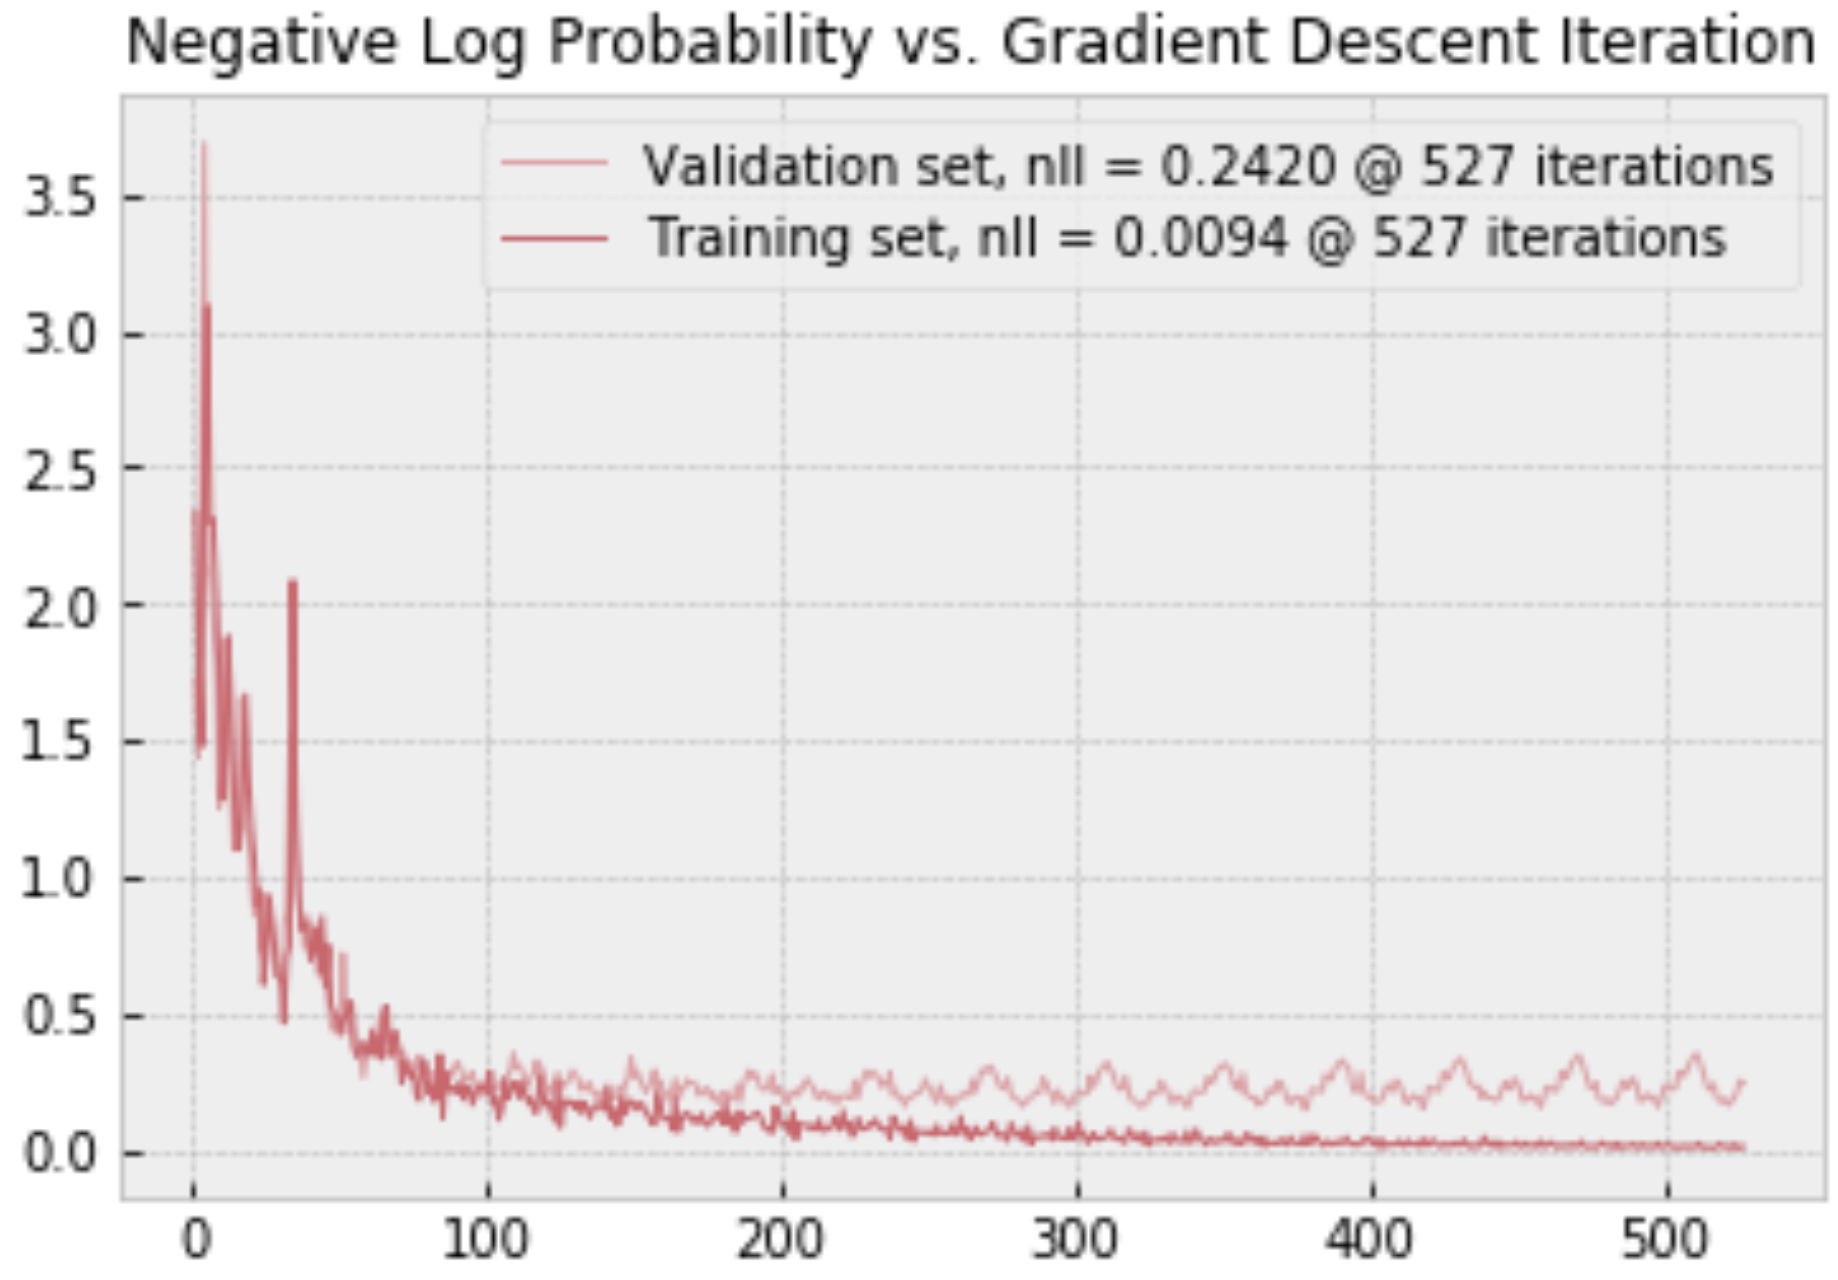
\includegraphics[width=\linewidth]{A4_1_1.png}
      \caption{Stricter convergence criteria}
    \end{subfigure}
    \begin{subfigure}[b]{0.45\linewidth}
      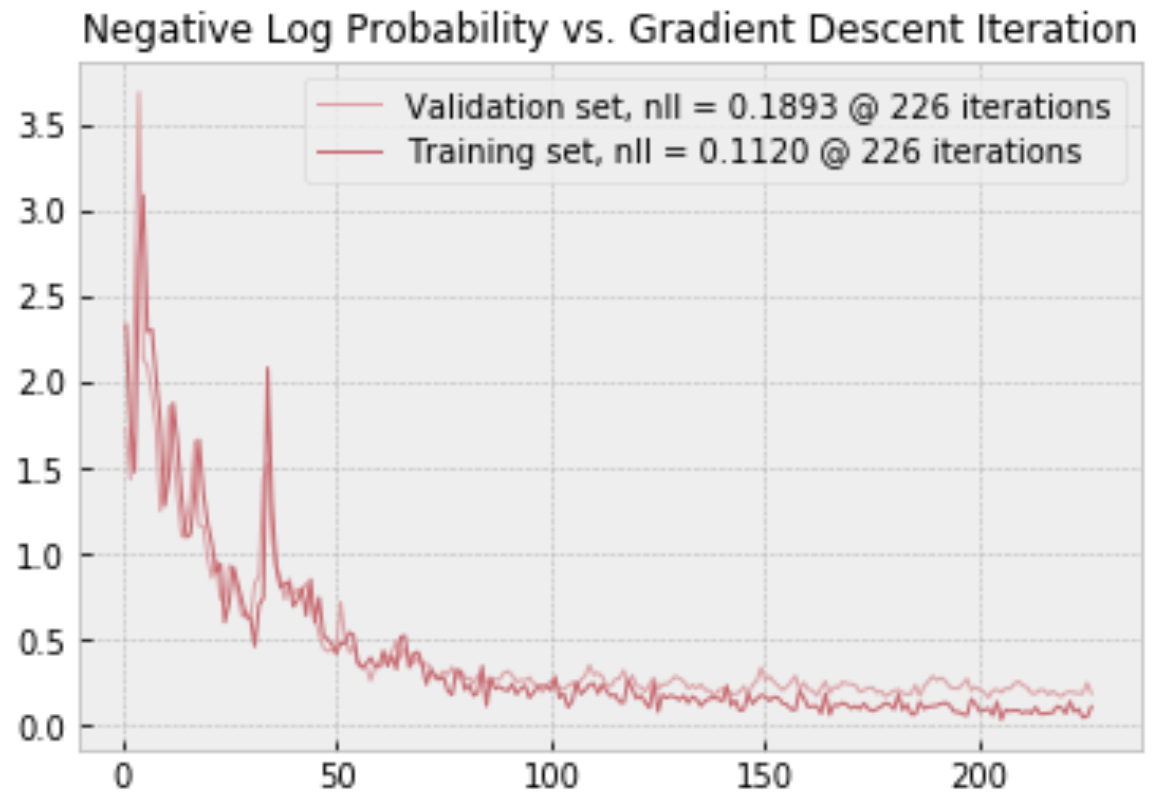
\includegraphics[width=\linewidth]{A4_1_2.png}
      \caption{Looser convergence criteria}
    \end{subfigure}
    \caption{The comparison between training and validation losses vs. iterations}
    \label{fig:Q1_1}
  \end{figure}

  Figure 1(a) is generated with the early stopping condition of any one or a combination of the followings: %\footnote{In alignment with the previous footnote, the early stopping criteria is also according to the values that are 20 iterations apart. This is why the convergence criteria seem loose (eg. smaller than the errorbound only twice is enough) -- if the comparison is made after every iteration, the criteria would be a lot stricter (eg. same criteria but requiring 20 times more repetition.)}:
  \begin{itemize}
    \item the difference between losses being smaller than the error bound for 40 times
    \item the difference between the past minimum and current loss being smaller than the error bound for 40 times
    \item the current loss is higher than the past minimum for 500 times
  \end{itemize}
  Under these criteria, the training set took about 500 iterations to converge to a very small negative likelihood of about 0.01 per datapoint. However, overfitting has clearly occured as the validation set started going flat and oscillating more heavily from about 200 iterations. Therefore, the 3rd stopping condition is loosened to the current loss being higher than the past minimum for 200 times instead of 500. From a comparison between Figure 1(a) and 1(b), we can conclude that \textbf{the train set loss would keep decreasing while that of the validation set would start flatting out at some point and oscillate, indicating an overfit in the model}, and that \textbf{with a losser early stopping/convergence condition and thus less iterations, the training set loss wouldn't be as low as that after more iterations, but the validation set one would be lower as there is less overfitting.}


\vspace{1cm}
\textbf{Performance with Different Configurations}

  3 different configurations are tested and compared. They have 10, 50, and 200 neurons per hidden layer, respectively. The learning rate of each is also adjusted to be the optimal and the performance both training and validation are summarized in Figure 2.

  % \begin{table}[!h]
  % \centering
  % \scalebox{0.9}{\begin{tabular}[t]{||r | c c c c c||}
  %   \hline
  %   \# Neurons per Hidden Layer & Learning rate & iterations  &  Negative Log Likelihood & Accuracy\\
  %   \hline
  %   10    & 0.1   & 0.333 & 103.783      & 0.8667 &\\
  %   50    & 0.25    & 0.8699 & 20.637       & 0.8669 &\\
  %   200   & 0.4    & 0.8703 & 10.504       & 0.8672 &\\
  %   \hline
  % \end{tabular}}
  % \caption{Iteration and validation performance with different configurations on MNIST dataset}
  % \end{table}

  % \begin{figure}[!h]
  %   \centering
  %   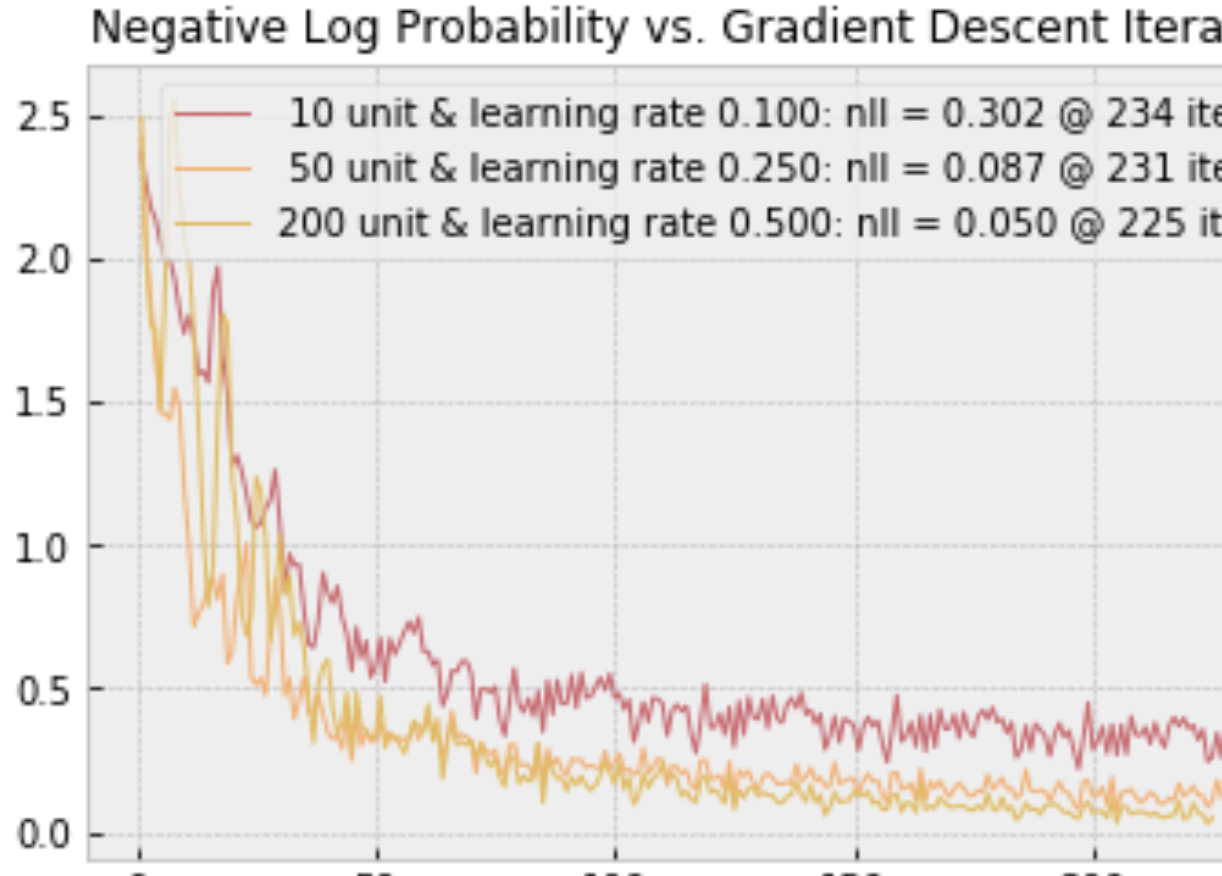
\includegraphics[width=0.6\linewidth]{A4_2.png}
  %   \caption{Training process with different network configurations}
  %   \label{fig:2}
  % \end{figure}

  \begin{table}[ht]
    \begin{minipage}[b]{0.35\linewidth}
      \centering
      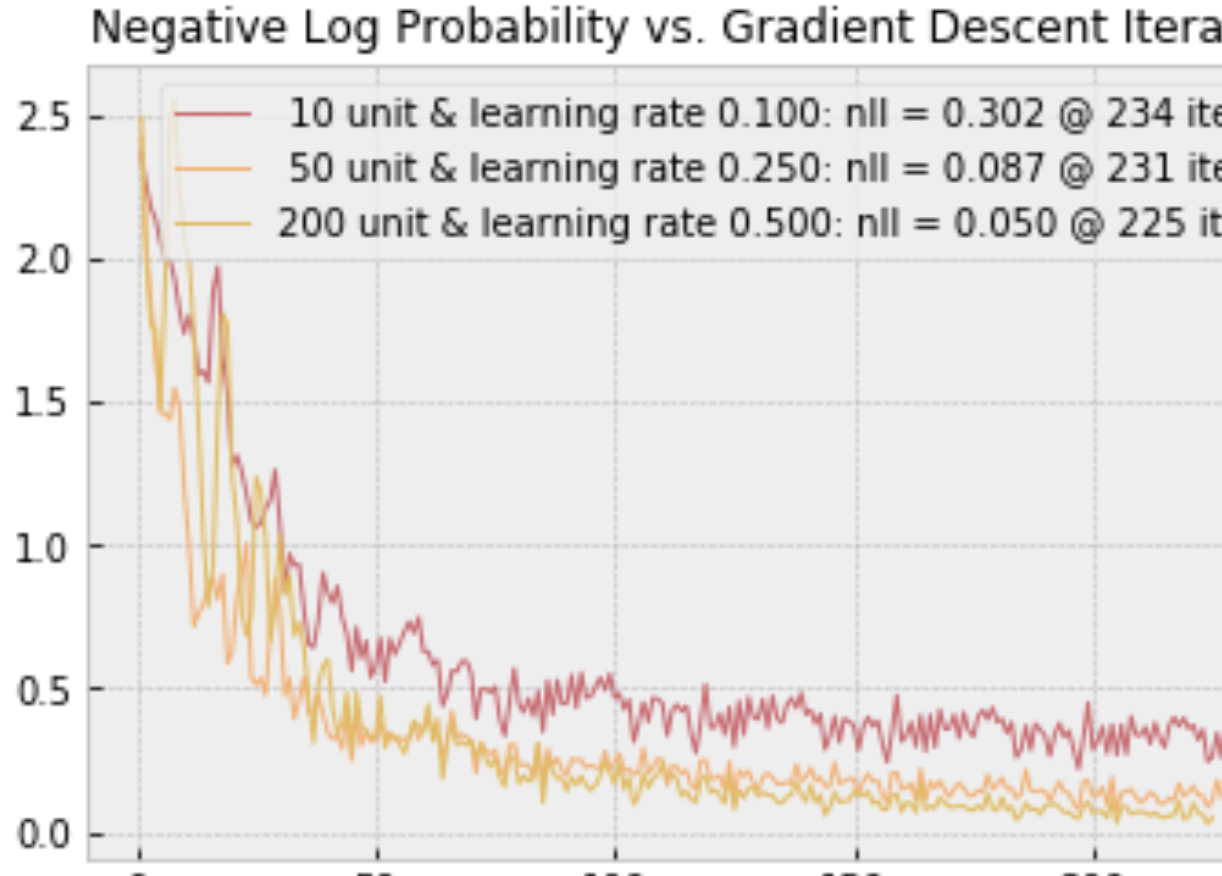
\includegraphics[width=\linewidth]{A4_2.png}
      \captionof{figure}{Training process with different network configurations}
      \label{fig:2}
    \end{minipage}
    \hfill
    \begin{varwidth}[b]{0.65\linewidth}
      \begingroup
      \setlength{\tabcolsep}{10pt} % Default value: 6pt
      \renewcommand{\arraystretch}{1} % Default value: 1
      \centering
      \scalebox{0.9}{\begin{tabular}{ l | r r r }
        \hline
        \hline
        \# Neurons & 10 & 50 & 200 \\
        \hline
        Learning Rate & 0.1 & 0.25 & 0.4 \\
        % \vtop{\hbox{\strut Iterations}\hbox{\strut on train set}} & 260 & 220 & 260\\
        Training Iterations & 260 & 220 & 260\\
        % \vtop{\hbox{\strut Negative Log Likelihood}\hbox{\strut on train set}} & 0.333 & 0.138 & 0.051 \\
        Negative Log Likelihood & 0.333 & 0.138 & 0.051 \\
        Accuracy & 88.8\% & 92.8\% & 94.5\% \\
        Loss & 0.381 & 0.209 & 0.170 \\
        \hline
        \hline
      \end{tabular}}
      \caption{Training process and validation performance corresponding to Figure 2}
      \label{table:1}
      \endgroup
    \end{varwidth}%
  \end{table}

  From both the training process and validation performance, it can be concluded that, the more neurons a fully-connected neural network had, the more accurate it will be to model the dataset. When there is only a few neurons (eg. 10 per layer), the learning rate will be required to be smaller in order for the training process to be stable, and it will end up performing poorer regardless, as there will not be enough features passing forward to represent the orginal features. The test results from the best configuration, 200 neurons per layer with a learning rate of 0.4, is \textbf{96.1\% accuracy and 0.129 average negative log likelihood}, and more details are presented and discussed in the last section of the report.


\vspace{1cm}
\textbf{Neuron Visualization}

  \begin{figure}[!hb]
    \centering
    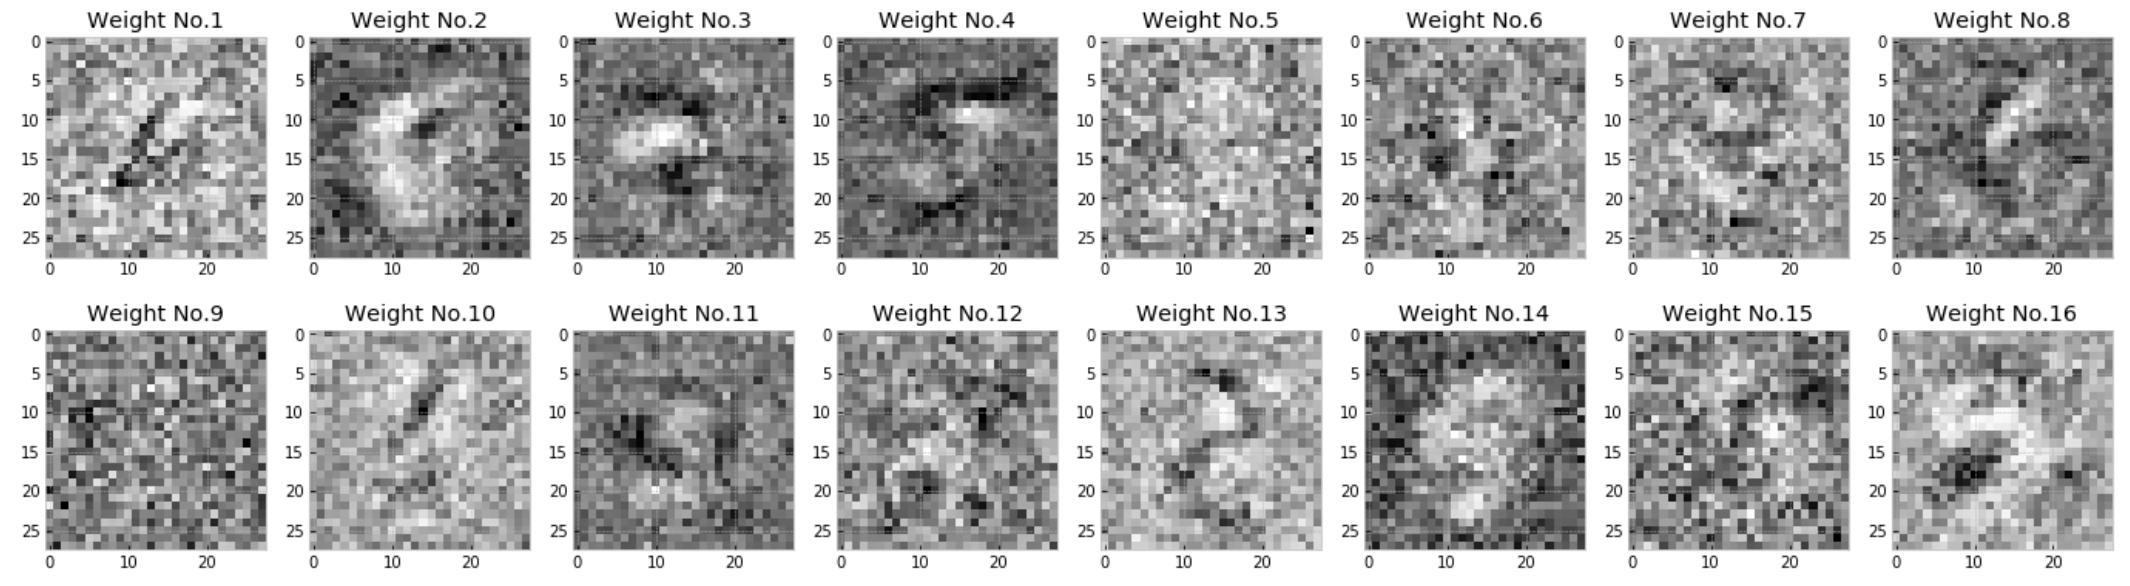
\includegraphics[width=\linewidth]{A4_3.png}
    \caption{First 16 neurons in the first hidden layer}
    \label{fig:3}
  \end{figure}

  The first layer weights of 16 neurons in the fully connected neural network are visualized in Figure 3. The darker the color, the larger the weight is. First and foremost, as this is a fully-connected layer, the weights essentially points out \textbf{"this (the darker region) is what should be examined in the next layer"}. In these 16 weights, No.1 had the triangular part of number "4", No.3 had a curve in "2", No.4 as a whole constructed a "5", No.8 is like "6", so on and so forth. Meanwhile, some other weights like No. 6, 7, 10, and 16 capture the edges and corners of numbers, which are also useful in distinguishing, for example, "8" and "9" who have a similar "circular upper part" but differ a lot in their bottom half.

\vspace{1cm}
\textbf{Images Leading to Inconfident Predictions}

  \begin{figure}[!h]
    \centering
    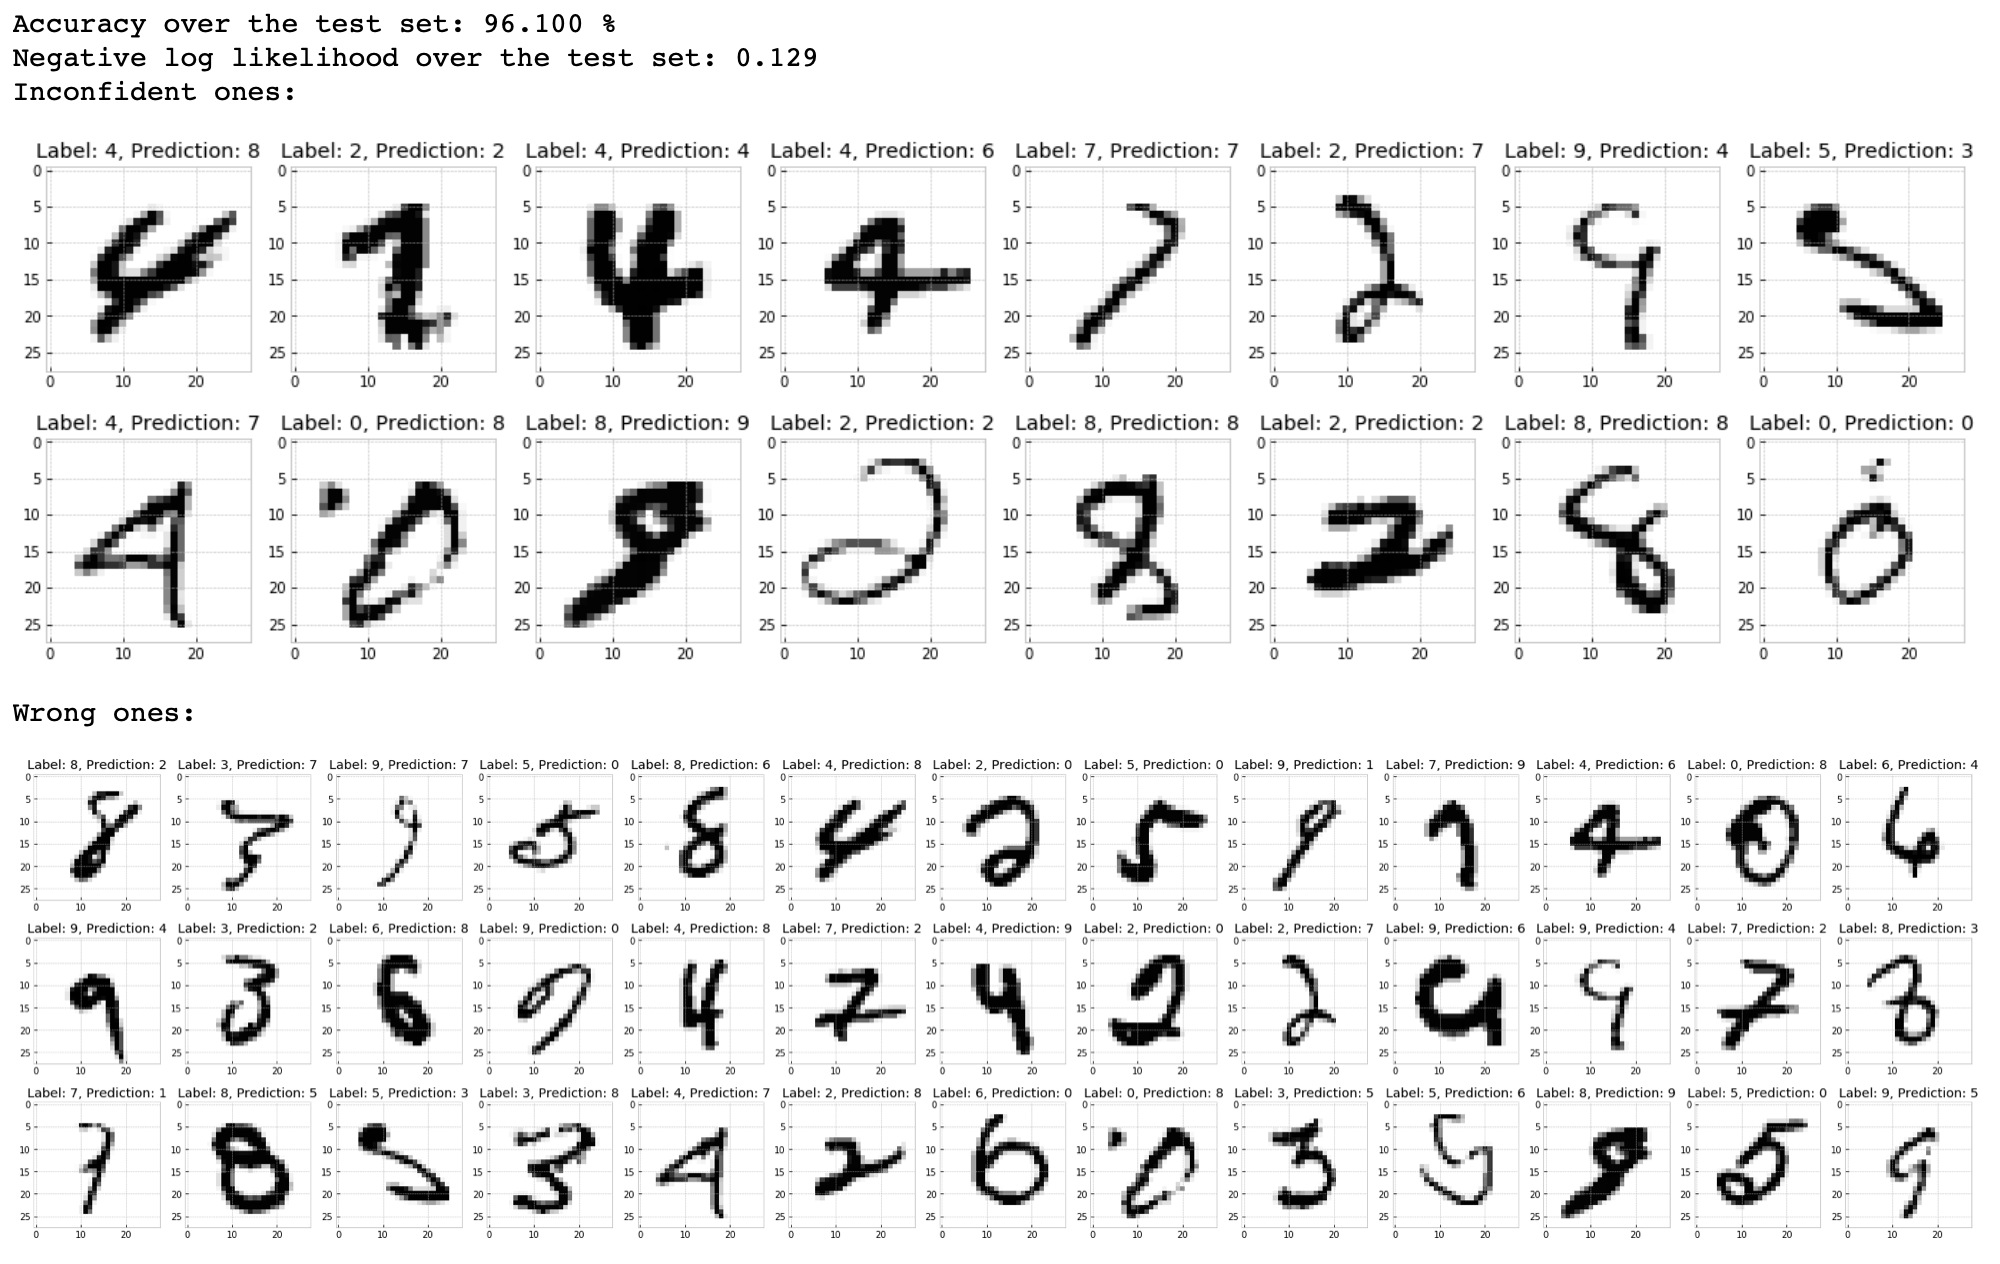
\includegraphics[width=\linewidth]{A4_4.png}
    \caption{Digits that lead to low likelihoods}
    \label{fig:4}
  \end{figure}
  
  The digits in Figure 4 led to condifence of lower than $0.125$, or a log likelihood of $-0.9$. From the previous section, we saw that the neural network chooses regions (continuous or not) of interest and biases the prediction on them. Basically, in every image of low confidence, there exist some regions that make them look like some other digits as much as their final guesses. For example, both "0"'s had an extra dot on top which could also appear in number "8", the first "8" in the second row had a line instead of a circle on the bottom, which is usually the case in "9". Another common triat of these numbers are that many of them are not straight, and the more tilted a number is, such as the first "4", the more likely its features seem to belong to other numbers. In fact, the aforementioned two problems are whidely found in the incorrectly predicted ones as well.

\end{document}
